% \iffalse
\let\negmedspace\undefined
\let\negthickspace\undefined
\documentclass[beamer]{IEEEtran}
\usepackage{cite}
\usepackage{amsmath,amssymb,amsfonts,amsthm}
\usepackage{algorithmic}
\usepackage{graphicx}
\usepackage{textcomp}
\usepackage{xcolor}
\usepackage{txfonts}
\usepackage{listings}
\usepackage{enumitem}
\usepackage{mathtools}
\usepackage{gensymb}
\usepackage{comment}
\usepackage[breaklinks=true]{hyperref}
\usepackage{tkz-euclide} 
\usepackage{listings}
\usepackage{gvv}                                        
\def\inputGnumericTable{}                                 
\usepackage[latin1]{inputenc}                                
\usepackage{color}                                            
\usepackage{array}                                            
\usepackage{longtable}                                       
\usepackage{calc}                                             
\usepackage{multirow}                                         
\usepackage{hhline}                                           
\usepackage{ifthen}                                           
\usepackage{lscape}
\usepackage[export]{adjustbox}

\newtheorem{theorem}{Theorem}[section]
\newtheorem{problem}{Problem}
\newtheorem{proposition}{Proposition}[section]
\newtheorem{lemma}{Lemma}[section]
\newtheorem{corollary}[theorem]{Corollary}
\newtheorem{example}{Example}[section]
\newtheorem{definition}[problem]{Definition}
\newcommand{\BEQA}{\begin{eqnarray}}
\newcommand{\EEQA}{\end{eqnarray}}
\newcommand{\define}{\stackrel{\triangle}{=}}
\theoremstyle{remark}
\newtheorem{rem}{Remark}
\begin{document}
\parindent 0px
\bibliographystyle{IEEEtran}

\title{GATE - BM 41}
\author{EE23BTECH11215 - Penmetsa Srikar Varma$^{}$% <-this % stops a space
}
\maketitle
\newpage
\bigskip

\renewcommand{\thefigure}{\theenumi}
\renewcommand{\thetable}{\theenumi}
\section*{Question}
Q41) A filter designed using opamps, resistors and capacitors as shown in figure.
Opamps are ideal with infinite gain and infinite bandwidth. If $\frac{\text{V}_0\brak{\text{S}}}{\text{V}_\text{i}\brak{\text{S}}}$ is an all-pass transfer function, the value of resistor R2 \brak{\text{in k}\Omega} is\\
\begin{figure}[h]
    \centering
    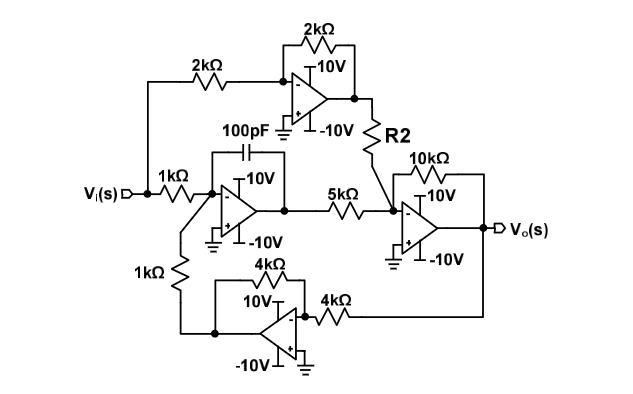
\includegraphics[scale=0.44]{figs/bm,41.png}
    \label{bm,41}
\end{figure}
\begin{center}
\end{center}
\brak{\text{A}}\ 1\\
\brak{\text{B}}\ 10\\
\brak{\text{C}}\ 5\\ 
\brak{\text{D}}\ 2\ \qquad\qquad\qquad\quad\qquad\qquad\qquad\qquad\brak{\text{GATE BM 2022}}
\section*{Solution}

\end{document}
